\chapter{Development}\label{ch:development}

\paragraph{Hardware testing} 

\section{Ultrasonic sensors}

First of the hardware we started testing the ultrasonic sensors.
For each of the sensors we built a voltage divider seen on the following figure.

\begin{figure}[h]
\centering
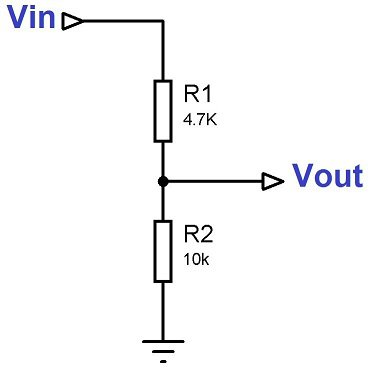
\includegraphics[width = 0.5\textwidth]{voltage1}
\caption{Voltage divider}
\label{fig::voltage1}
\end{figure}

The values of the resistors are calculated by the following equation:
\begin{equation} \label{voltagedivider} 
{V}_{out}={V}_{in}*{R}_{2}/({R}_{1}+{R}_{2})
\end{equation}

We tried all the sensors out seperately by connecting them 1 by 1 to the raspberry and ran the test code.

\begin{lstlisting}
import RPi.GPIO as GPIO
import time
GPIO.setmode(GPIO.BCM)

TRIG = 23
ECHO = 24

print "Measuring distance"

GPIO.setup(TRIG, GPIO.OUT)
GPIO.setup(ECHO, GPIO.IN)

while True:
	GPIO.output(TRIG, False)
	print "W8ing on da sensor"
	time.sleep(2)

	GPIO.output(TRIG, True)
	time.sleep(0.00001)
	GPIO.output(TRIG, False)

	while GPIO.input(ECHO)==0:
		pulse_start = time.time()

	while GPIO.input(ECHO)==1:
		pulse_end= time.time()

	pulse_duration = pulse_end - pulse_start

	distance = pulse_duration * 17150
	distance = round(distance, 2)

	print "Distance:%d",distance

\end{lstlisting}

Each of the sensors worked correctly while connected seperately so we moved on to try them out all of them at the same time.
For that we connected all of the ultrasonic sensors to the raspberry and tried them out.
For testing all of them we included some filtering aswell, because while taking every reading we saw that some of the values where off the chart high.
High values was most probably due to the noise or just some random jittering.
Our filter is made to take three readings at the time and then calculate the average.

\begin{lstlisting}
def readsensor(PIN):
	for x in range(0, 2):
		read_time_start1 = time.time()
		GPIO.output(TRIG, True)
		time.sleep(pulse)
		GPIO.output(TRIG, False)

		while GPIO.input(PIN)==0:
			pulse_start = time.time()

		while GPIO.input(PIN)==1:
			pulse_end= time.time()

		pulse_duration[x] = pulse_end - pulse_start
		time.sleep(0.05-(time.time()-read_time_start1))

	distance = sum(pulse_duration)/measurment_count* SPEED_OF_SOUND
	distance = round(distance, 2)
	print distance
while True:
	readsensor(ECHOF)
	readsensor(ECHOR)
	readsensor(ECHOL)
	
\end{lstlisting}

As you can see from the code above we made sure that every reading takes exactly 0.05 seconds.
This will help us make every cycle evenly long and we can predict the total time that the program runs the whole cycle.
After applying the filter we saw that the readings became alot more percise and consistent.
Therefore the time for the sensor reading loop becomes 3*0,05s=0,15s.

\section{DC motors}

For testing the dc motors we drove the motors in forward gear and in backward gear through the driver we are useing.
Below you can see the script we used to conduct the testing of the motors.

\begin{lstlisting}
GPIO.setmode(GPIO.BCM)
GPIO.setup(StepPinForward, GPIO.OUT)
GPIO.setup(StepPinBackward, GPIO.OUT)

def forward(x):
    GPIO.output(StepPinForward, GPIO.HIGH)
    print "forwarding running  motor "
    time.sleep(x)
    GPIO.output(StepPinForward, GPIO.LOW)

def reverse(x):
    GPIO.output(StepPinBackward, GPIO.HIGH)
    print "backwarding running motor"
    time.sleep(x)
    GPIO.output(StepPinBackward, GPIO.LOW)

print "forward motor "
forward(5)
print "reverse motor"
reverse(5)

print "Stopping motor"
GPIO.cleanup()

\end{lstlisting}

As you can see from the code it runs one of the two motors first forward for 5 seconds and then backwards for 5 seconds.
For the second motor we just changed the pin numbers(StepPinForward and StepPinBackward).
